\documentclass[journal]{IEEEtran}
\usepackage{amsmath,booktabs,multirow,graphicx,url}
\usepackage[hidelinks]{hyperref}

\begin{document}
\title{What an SDN Controller Can Actually Observe:\\
A Measurement and Validity Study of the InSDN OpenFlow Control Channel}

\author{\IEEEauthorblockN{Adhyan Jain\IEEEauthorrefmark{1}, Atharva Sheersh Pandey\IEEEauthorrefmark{1} and Kshitij Manikshete\IEEEauthorrefmark{1}}
\IEEEauthorblockA{Vellore Institute of Technology (VIT), Vellore, India\\
adhyan.jain2024@vitstudent.ac.in, atharva.sheersh2024@vitstudent.ac.in, kshitij.rahul2024@vitstudent.ac.in}
\thanks{\IEEEauthorrefmark{1}All three authors contributed equally to this work.}}

\maketitle

\begin{abstract}
SDN intrusion-detection research is evaluated mostly on benchmark CSVs of CICFlowMeter 5-tuple flow records,
computed offline from packet captures at the attacked host. Whether an SDN controller can observe anything
resembling these records is rarely checked. We check it inside the benchmark itself. InSDN, a widely used SDN
intrusion dataset, also published packet captures of its ONOS controller's OpenFlow~1.3 control channel; we parse
all 44 of them (11 benign and 33 attack sessions across seven attack classes). In every flow-statistics reply, and in
all 3\,827 FlowMods, in these captures the controller's flow entries match only on \texttt{eth\_type} or
\texttt{(in\_port, eth\_src, eth\_dst)}; none matches IP addresses or transport ports, so the dataset's labelled
5-tuple flows are not counters the controller can read. What the controller does receive is a dense PacketIn stream: in 9 of 12 attack
scenarios, between 0.68 and 1.29 PacketIns per data packet seen at the target. Using only this controller-observable
view, small models reach a balanced accuracy of 0.946 on unseen captures under capture-grouped cross-validation
(against 0.616 for a PacketIn-rate threshold) and 0.89--1.00 on all six withheld attack families (best
single-feature threshold 0.70--0.97); logistic regression matches the neural network overall. We then show that these numbers cannot be read as attack-detection accuracy: InSDN records
benign and attack traffic in separate sessions and its labels cover only part of the controller-visible traffic, so
within attack sessions a trivial ``any IP PacketIn'' rule scores 0.995 under strict labels, and our session probes
cannot separate session identity from unlisted attack traffic. We report this as a validity threat for controller-side
evaluation on InSDN. Finally, a benign-traffic Mininet/Ryu case study (10 runs per mode on one switch, 10 on a three-switch chain) shows that the forwarding
application sets what the controller observes: per-flow forwarding produced about 10\,400 TCP PacketIns per run against
about 12 for MAC-pair forwarding (at least 665$\times$ in every paired run, for both timeouts; at least 391$\times$ on three switches), and a 2\,s idle timeout reduced the
IP-specific entries a 1\,s poller sees from $153.1\pm2.4$ to $36.9\pm0.5$ per reply. A first campaign with a flawed
application, in which ping and ARP entries shadowed TCP, understated the PacketIn effect by more than two orders of
magnitude; we report both. Ryu's unmodified \texttt{simple\_switch\_13} application, run as a second controller in five
captures, also installed only MAC-pair entries (86 of 91 FlowMods; none with IP or transport fields). Second, we audit the evaluation protocol. The concern that random splits and identifier columns inflate NIDS scores is known for non-SDN
benchmarks; we quantify it with one pipeline on two datasets. On InSDN a random flow-level split gives 0.9998 balanced accuracy, whereas holding out source hosts gives
$0.907\pm0.085$ (worst split 0.66); on CICIDS2017 the values are 0.9917 and $0.641\pm0.056$; IP addresses and ports alone give at least 0.9999 on both, and
48.7\% of InSDN's random-split test rows duplicate a training row, but removing all exact duplicates leaves the random-split score at 0.9998, and the host-held-out drop persists when every attack class is present in training (0.939), so duplicates do not explain it. Of nine InSDN papers read in full, none reports a host-grouped split and three use identifier columns as inputs, so their protocols cannot rule out this leakage;
this does not show their reported numbers are wrong. A recipe replication with one classifier, approximating four published feature choices, scores at least 0.9998 binary balanced accuracy under a random split and 0.856--0.943 under a host-grouped split (a stress test, since grouping also changes class composition). A third dataset, UKMDDoSDN, could not be used.
\end{abstract}

\begin{IEEEkeywords}
Software-defined networking, intrusion detection, OpenFlow, ONOS, InSDN, telemetry, evaluation methodology
\end{IEEEkeywords}

\section{Introduction}
Machine-learning intrusion detection for software-defined networks (SDN) is commonly motivated by the controller's
global view~\cite{kreutz2015sdn}. In practice, evaluation rarely involves a controller: models are trained and
tested on flow records computed by CICFlowMeter~\cite{lashkari2017cicflowmeter} from packet captures at the attacked
hosts, then described as SDN detectors. InSDN~\cite{elsayed2020insdn} is a prominent example; its CSV release of
$\sim$344k labelled bidirectional 5-tuple flows with 80+ statistical features is widely used as an SDN benchmark.

A controller cannot compute those features for flows it does not see in full. An OpenFlow~1.3 controller~\cite{onf2012openflow13} observes PacketIn
messages for packets that miss the flow table, flow-statistics replies with packet and byte counters for whatever
entries its forwarding application installed, and its own FlowMod/PacketOut decisions. Inter-arrival-time moments,
per-direction length statistics and flag counts are not in that vocabulary. Earlier work criticised benchmark flow
features for diverging from real flow metering~\cite{engelen2021troubleshooting,pinto2025flowexporter,pekar2024integrity},
argued for standard feature sets~\cite{sarhan2022standard}, and measured the cost of assuming complete
flows~\cite{pekar2024partial}; a recent dataset records control-plane telemetry on a new testbed~\cite{lansdnnids2026}.
Controller-side detectors based on PacketIn behaviour exist~\cite{braga2010lightweight,mousavi2015early,shin2013avantguard,wang2015floodguard,dhawan2015sphinx},
but they are evaluated on their own traffic. We found no work that measures, inside InSDN, what the
controller observed, or that evaluates detection restricted to that view (our searches were conducted in October
2026; they are evidence, not proof, of absence).

InSDN's authors also captured the ONOS~\cite{berde2014onos} controller interface during every scenario. We analyse
these captures and make seven contributions; the first two are the main ones:
\begin{enumerate}
\item \textbf{A measured observability gap (\S\ref{sec:gap}).} Across all flow-statistics replies, only two match
structures occur and none involves IP or transport fields (also true of all 3\,827 FlowMods); in 9 of 12 scenarios the
controller receives 0.68 to 1.29 PacketIns per target packet.
\item \textbf{A quantified evaluation-validity audit (\S\ref{sec:audit}).} With one pipeline on InSDN and CICIDS2017, random flow splits give
0.9998 and 0.9917 balanced accuracy, while holding out source hosts gives $0.907\pm0.085$ and $0.641\pm0.056$, and IPs and ports alone give at least 0.9999. The
general leakage concern is known~\cite{engelen2021troubleshooting,flood2024baddesign}; what is new is the paired, quantified gap on an SDN dataset, and an audit of the protocols of 12 published papers (10 read in full; nine of them on InSDN), plus a recipe replication on InSDN in which four published-style feature recipes score at least 0.9998 binary balanced accuracy under a random split but 0.856--0.943 under a host-grouped split (Table~\ref{tab:recipe}).
\item \textbf{A reproducible control-channel pipeline (\S\ref{sec:method}).} An OpenFlow~1.3 parser and window
featuriser for the 44 captures with reported parser loss, and window labels grounded in InSDN's own flow labels.
\item \textbf{Detection from the controller's view, as a feasibility result (\S\ref{sec:results}).} Evaluated on
unseen captures, withheld attack families and across the two target deployments, against threshold heuristics and
simpler models, over 10 seeds.
\item \textbf{A validity analysis of the controller-view scores (\S\ref{sec:confound}).} Under InSDN's design, the detection scores cannot be
separated from session recognition and label coverage; we quantify what a trivial rule achieves and what our probes
can and cannot show.
\item \textbf{A forwarding-application case study (\S\ref{sec:live}).} In a Mininet/Ryu testbed with benign traffic,
per-flow forwarding produces about 10\,400 TCP PacketIns per run against about 12 for MAC-pair forwarding, and the
idle timeout sets how many entries a poller sees; a first campaign with a flawed application understated this effect.
\item \textbf{A second-controller check and a reproducibility package (\S\ref{sec:live} and Data and Code Availability).} Ryu's unmodified
learning-switch application also installs only MAC-pair entries, and every result file, table and quoted number can be
regenerated and compared automatically from hashed raw captures.
\end{enumerate}

\section{Background and Related Work}
\textbf{What an OpenFlow controller observes.} Under reactive forwarding, the first packet of an unmatched flow
reaches the controller as a PacketIn carrying the packet's headers; the controller answers with a PacketOut and
optionally installs an entry via FlowMod. It can poll per-entry packet and byte counters with multipart
flow-statistics requests~\cite{onf2012openflow13}. Which entries exist, and hence what the counters mean, is decided
by the forwarding application, not by the IDS.

\textbf{Benchmark realism and evaluation pitfalls.} Sommer and Paxson~\cite{sommer2010outside} and Arp et
al.~\cite{arp2022dos} catalogue pitfalls of ML-based detection, including spurious correlations. Engelen et
al.~\cite{engelen2021troubleshooting} found labelling and flow-construction errors in CICIDS2017; Pekar and Jozsa
studied dataset integrity~\cite{pekar2024integrity} and train/test flow completeness~\cite{pekar2024partial};
Pinto et al.~\cite{pinto2025flowexporter} showed detectors depend on the flow exporter; Sarhan et
al.~\cite{sarhan2022standard} argued for standard NetFlow feature sets. These concern flow-record features; none asks
what an SDN controller can observe.

\textbf{Evaluation protocol in InSDN detection papers.} Published InSDN detectors report accuracies of 96\% to 99.7\%.
Flood et al.~\cite{flood2024baddesign} and Engelen et al.~\cite{engelen2021troubleshooting} describe split leakage and identifier shortcuts on non-SDN benchmarks; Section~\ref{sec:audit} extends that
to InSDN with a paired measurement and summarises the protocols of the InSDN papers we could read in full (e.g.\ Towhid et al.~\cite{towhid2023early} divide all flows 70:30; grouping by capture or session is not mentioned).

\textbf{Controller-side detection and control-plane data.} PacketIn and flow-table signals have long been used to
detect flooding at the controller~\cite{braga2010lightweight,mousavi2015early} and to protect it~\cite{shin2013avantguard,wang2015floodguard,dhawan2015sphinx}.
Arévalo-Herrera et al.~\cite{lansdnnids2026} release a dataset that pairs traffic features with control-plane
metrics (PacketIn and FlowMod counts) collected on an OpenDaylight testbed. Their ablation reports that removing the OpenFlow features lowers link-fabrication F1 from 0.97 to 0.19 on
that dataset, which supports the premise that control-plane telemetry carries signal for SDN-specific attacks; our results neither
confirm nor contradict it, because we study volumetric and scan traffic on a different testbed. The UKMDDoSDN
dataset~\cite{ukmddosdn2025} (Ryu, DDoS) ships PCAPs, but the two we fetched (SYN and UDP flood, 310\,k packets in total) contain no
OpenFlow packets at all (Appendix~\ref{app:ukm}), so they cannot support a control-channel analysis. Our work is complementary: we do not
introduce a new dataset, but characterise and use the controller-side captures already shipped with InSDN, so
results remain comparable with the large body of InSDN work.

\section{Threat Model and Scope}\label{sec:threat}
\textbf{Defender.} The detector runs at (or beside) an SDN controller and may read only what the OpenFlow~1.3 control
channel carries: PacketIn, PacketOut, FlowMod, FlowRemoved and flow-statistics messages. It has no tap on host links and
no packet captures from the data plane. We assume the controller's forwarding application is fixed and known.

\textbf{Attacker.} The attacker is an end host that sends volumetric (DoS/DDoS), scanning, brute-force, exploit, web or
botnet traffic through the switch. We do not consider an attacker who attacks the controller or the control channel
itself (e.g.\ spoofed PacketIn floods aimed at saturating it), who knows the detector, or who adapts traffic to mimic
benign PacketIn statistics; the evaluation is therefore a measurement of what is observable and separable in recorded
benchmark traffic, not a robustness claim.

\textbf{Out of scope.} Inline operation, mitigation, latency, encrypted-payload effects, and attacks on switches.
The paper makes claims about (i) what two forwarding applications install, (ii) separability within InSDN's
captures, and (iii) validity of that separability as detection evidence.

\section{What the Controller Sees in InSDN}\label{sec:gap}
\textbf{Data.} InSDN~\cite{elsayed2020insdn} was generated with Mininet hosts and an Open vSwitch switch controlled by
ONOS; attacks target a Metasploitable-2 VM or the OVS host. Besides the CSVs, the authors published PCAP groups
(\emph{Normal}, \emph{Metasploitable-2}, \emph{OVS}) recorded at the target and at the controller interface. We
downloaded them from the dataset's institutional host; the Metasploitable-2 and OVS archives passed ZIP integrity
checks, and for the Normal archive we fetched only the controller captures through HTTP range requests on its ZIP
members, each checked against its recorded size. SHA-256 hashes of the 44 captures and the two full archives are
released with the code (\texttt{capture\_hashes.sha256}).
The 44 controller captures (\texttt{*ONOS*}) are the subject of this paper (Table~\ref{tab:inventory}).

\textbf{Granularity.} We decoded every OpenFlow~1.3 multipart flow-statistics reply in all 44 captures. Only two
match structures occur: \texttt{eth\_type} (the controller's default punt rules; 80\,464 entry observations) and
\texttt{(in\_port, eth\_src, eth\_dst)} (reactive forwarding; 24\,437 observations). No entry matches IP addresses
or transport ports. A 5-tuple flow, the unit InSDN labels, is therefore never a counter the controller can read; a
MAC-pair entry aggregates every flow between two hosts. The 3\,827 FlowMods the controller sent show the same: 3\,811
match \texttt{(in\_port, eth\_dst, eth\_src)}, 16 match \texttt{eth\_type}, and none has IP or transport fields, so a
short-lived 5-tuple entry cannot have slipped between two polls. This describes the ONOS forwarding configuration used
in InSDN; it is not a property of OpenFlow in general.

\textbf{The PacketIn stream.} Table~\ref{tab:gap} pairs each attack scenario's target-side captures with its
controller captures. In 9 of 12 scenarios the controller receives between 0.68 and 1.29 PacketIns per data packet
recorded at the target. Two Metasploitable-2 scenarios show 3.9 and 15.7. The OVS DDoS scenario shows 0.08 (6.5M
target packets against 541k PacketIns), consistent with control-channel saturation under a spoofed flood; we did not
test this directly. The two sides are separate recordings and their alignment is unverified, so ratios are
indicative, not exact per-packet counts. The Normal group has no target-side captures, so we have no such ratio for
benign traffic. Because each PacketIn carries the packet's headers, the 5-tuple is visible to the controller per
packet, but never as a per-flow counter.

\begin{figure}[t]
\centering
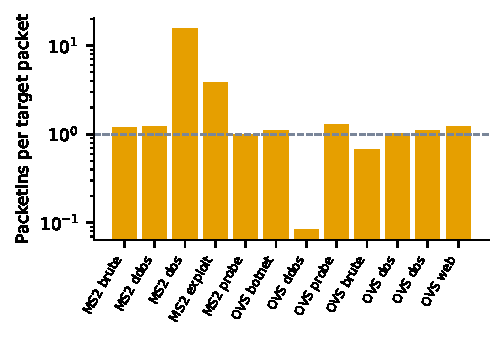
\includegraphics[width=\columnwidth]{fig_packetin_ratio.pdf}
\caption{PacketIns received by the ONOS controller per packet seen at the target, by attack scenario (MS2: Metasploitable-2 target, OVS: OVS target). The dashed line marks one PacketIn per packet. Data: \texttt{gap\_attack\_v2.json}.}\label{fig:ratio}
\end{figure}

\textbf{Implication.} A model trained on InSDN's CSV consumes statistics (inter-arrival moments, per-direction length
moments, flag counts per 5-tuple) that this controller never receives. The deployable signal is the PacketIn header
stream plus coarse MAC-pair counters, which we use directly.

\section{Controller-Observable Detection}\label{sec:method}
\textbf{Parsing.} We reassemble each TCP direction of the control channel (port 6653), split it into OpenFlow
messages by header length, and decode PacketIn (with the embedded Ethernet frame), PacketOut, FlowMod, FlowRemoved
and flow-statistics replies. On a header desynchronisation the parser scans forward for the next position that
starts a chain of two plausible headers. Over the 44 captures it decoded 7\,381\,679 messages, resynchronised
134 times and discarded 12\,217 bytes; reassembly is in arrival order with sequence-number deduplication only, so
these loss figures are a lower bound. (A first version that dropped its whole buffer on every desync discarded
44.6\,MB and lost up to $\sim$90\% of PacketIns on some DDoS captures; all reported results use the corrected parser.)
182\,153 PacketIns are truncated by the switch to a header prefix; their headers still parse and labelling is
unaffected.

\textbf{Features.} For each window of $W{=}1$\,s we compute 22 controller-observable features: counts of PacketIn,
PacketOut, FlowMod, FlowRemoved and statistics replies; from PacketIn frames, the number of distinct source and
destination MACs, IPs and destination ports, TCP/UDP/ICMP/ARP fractions, the SYN-only fraction of TCP, mean frame
length, and the entropies of source IP and destination port; and, from consecutive statistics replies of the same
entry, the number of entries and the sum and maximum of packet and byte deltas. The model input concatenates the
current and three previous windows ($\log(1{+}x)$ transformed).

\textbf{Labels grounded in the dataset (strict).} Labelling a window by the capture it came from would mark every
quiet window of an attack session as an attack. Instead we label each PacketIn by matching its 5-tuple (either
direction) to InSDN's CSV Flow IDs. A window is an attack window iff it contains at least one PacketIn matching an
attack flow. In attack captures, a window with no attack match but with PacketIns of unmatched IP traffic is
ambiguous and is excluded from training and scoring; benign captures keep all windows. This is restrictive and
sparse: the CSV covers only part of each capture, so after exclusion brute force, exploit and web keep only 6, 12 and
12 attack windows, and DDoS 55 of 499 (Table~\ref{tab:inventory}). As \S\ref{sec:confound} shows, the exclusion also
removes exactly the hard negatives of attack sessions.

\textbf{Detectors and baselines.} A two-layer MLP (64--32 units, dropout, class-weighted cross-entropy, 40 epochs)
trained on an NVIDIA RTX 4060 GPU; a logistic-regression model on the same inputs; a single-window MLP; ablations to
PacketIn-derived or flow-statistics-derived features; and four single-feature thresholds fitted on the training
folds (PacketIn rate, a causal per-capture-normalised burst rate, source-IP entropy, destination-port entropy). A gradient-boosted-tree baseline (XGBoost, trained on the GPU) uses the same inputs, and a host-side baseline uses InSDN's
own flow-CSV features (below).

\textbf{Protocol.} No capture appears in both training and test. (A)~5-fold cross-validation grouped by capture file
and stratified by class; (B)~leave-one-attack-family-out, with DoS and DDoS withheld together as ``flood''; (C)~cross-deployment,
training on one target group and testing on the other, with disjoint benign captures; (D)~session probes; (E)~a
label-shuffle sanity check. Every experiment uses 10 seeds (fold assignment and initialisation). We report mean and
95\% $t$-interval over seeds, which reflects fold and initialisation variability on the same 44 captures, not
sampling of new testbeds, and a stratified cluster bootstrap over captures for pooled window counts (a CI of pooled
window BAcc, dominated by the many benign windows, hence not comparable to the seed mean). Folds are grouped by
capture file, not by scenario: variants of one scenario (e.g.\ SYN, UDP and ICMP DDoS) can fall on both sides of a
fold, so (A) is optimistic; (B) and (C) are the scenario-held-out tests. Balanced accuracy (BAcc) is the headline
because classes are imbalanced.

\section{Results}\label{sec:results}
\textbf{Unseen captures (Table~\ref{tab:cv}).} The controller-observable MLP reaches BAcc 0.946 with a window
false-positive rate of 0.001. The PacketIn-rate threshold, the usual SDN flooding heuristic, reaches only 0.616; a
likely reason is that benign sessions also produce heavy PacketIn volume, but we cannot verify this against a
target-side benign ratio (\S\ref{sec:gap}). Entropy thresholds do better (0.839--0.852) but stay below the learned
models. PacketIn features carry the signal (0.943 alone); flow-statistics features alone reach 0.699 at 1\,s with a
high FPR (0.918 at 5\,s), consistent with MAC-pair counters being coarse. A logistic-regression model (0.939) and a single-window MLP (0.934) are
close to the full model overall, so history and non-linearity add little here, although logistic regression differs
on some withheld families (e.g.\ botnet 0.803 vs.\ 0.932). The capture-level bootstrap (Table~\ref{tab:boot}) is
wider than the seed intervals and pools windows, so it is dominated by benign windows; there the entropy thresholds
look competitive with the learned models, and the seed-level comparisons are the more informative ones. The
label-shuffle control (each capture given another capture's window-label sequence) gives BAcc $0.512\pm0.054$ at
1\,s and $0.508\pm0.067$ at 5\,s, i.e.\ chance; it shows the pipeline does not read labels from where it should not,
and says nothing about label--feature overlap or session identity.

\textbf{Withheld attack families (Table~\ref{tab:family}).} With a family absent from training, the MLP beats the best
single-feature threshold on flood (0.936 vs.\ 0.814), probe (0.997 vs.\ 0.970) and web (0.904 vs.\ 0.699), ties on
brute force and exploit, and loses on botnet (0.932 vs.\ 0.965; one capture). The best threshold is chosen per
family in hindsight, which favours the baseline, and brute force, exploit and web rest on 6--12 attack windows.

\textbf{Across deployments (Table~\ref{tab:cross}).} Training on OVS-target sessions and testing on
Metasploitable-2 sessions gives 0.990 (best threshold 0.947); the reverse gives 0.905 (best threshold 0.866).

\textbf{Window length.} With $W{=}5$\,s (strict labels, 10 seeds) the picture is consistent: BAcc 0.958 for the MLP
(logistic regression 0.961, single window 0.944) and the PacketIn-rate threshold at 0.527. Flow-statistics features
alone improve to 0.918, since a longer window usually spans a counter poll. Cross-deployment gives 0.978 (OVS
$\rightarrow$ Metasploitable-2; best threshold 0.910) and 0.895 (reverse; 0.860).

\textbf{Host-side baseline.} For contrast, the usual flow-CSV protocol applied to InSDN's own CICFlowMeter features
(343\,889 flows, 78 numeric features, benign vs.\ any attack, XGBoost on the GPU, 10 seeds of stratified 70/30 row splits)
reaches BAcc $0.9998\pm0.00003$. This is not a comparison on the same traffic or the same units: rows are flows, not windows;
rows of one session fall on both sides of the split; and these features are not available to a controller. It shows that
the usual benchmark protocol is far easier than capture-grouped evaluation of the controller view; it should not be read as
the controller-side detector being 5 points worse.

\begin{table}[t]
\caption{Controller captures (1\,s windows). Under strict labels, ambiguous windows of attack captures are excluded (``kept'').}
\label{tab:inventory}
\centering\footnotesize\setlength{\tabcolsep}{3pt}
\begin{tabular}{lrrrrr}
\toprule
Class & Captures & Windows & Kept & Attack win. & PacketIns \\
\midrule
Normal & 11 & 33,283 & 33,283 & 0 & 789,569 \\
DoS & 11 & 861 & 805 & 456 & 845,362 \\
DDoS & 6 & 499 & 184 & 55 & 1,340,347 \\
Probe & 4 & 5,968 & 2,921 & 1,965 & 621,986 \\
Brute force & 4 & 604 & 359 & 6 & 5,564 \\
Exploit & 4 & 88 & 71 & 12 & 332 \\
Web & 3 & 636 & 275 & 12 & 1,199 \\
Botnet & 1 & 160 & 152 & 83 & 1,002 \\
\bottomrule
\end{tabular}
\end{table}

\begin{table}[t]
\caption{Target-side traffic vs.\ controller observations per scenario (ratio = PacketIns per target packet).}
\label{tab:gap}
\centering\footnotesize
\begin{tabular}{llrrrr}
\toprule
Group & Scenario & Target pkts & 5-tuples & PacketIns & Ratio \\
\midrule
Metasp. & Brute force & 1,311 & 295 & 1,574 & 1.20 \\
Metasp. & DDoS & 652,495 & 651,083 & 799,253 & 1.22 \\
Metasp. & DoS & 13,078 & 989 & 205,198 & 15.69 \\
Metasp. & Exploit & 86 & 18 & 332 & 3.86 \\
Metasp. & Probe & 507,650 & 51,150 & 510,194 & 1.01 \\
OVS & Botnet & 902 & 164 & 1,002 & 1.11 \\
OVS & DDoS & 6,510,923 & 6,508,402 & 541,094 & 0.08 \\
OVS & Probe & 86,705 & 79,021 & 111,792 & 1.29 \\
OVS & Brute force & 5,892 & 1,112 & 3,990 & 0.68 \\
OVS & App.\ DoS & 299,625 & 41,738 & 308,681 & 1.03 \\
OVS & Net.\ DoS & 304,886 & 20,979 & 331,483 & 1.09 \\
OVS & Web & 987 & 176 & 1,199 & 1.21 \\
\bottomrule
\end{tabular}
\end{table}

\begin{table}[t]
\caption{Unseen captures, grouped 5-fold CV, $W{=}1$\,s, strict labels, 10 seeds (mean{\scriptsize$\pm$}95\% CI over seeds).}
\label{tab:cv}
\centering\footnotesize\setlength{\tabcolsep}{3pt}
\begin{tabular}{lccc}
\toprule
Method & BAcc & Recall & FPR \\
\midrule
MLP, all features & 0.946{\scriptsize$\pm$0.016} & 0.893 & 0.001 \\
MLP, PacketIn features only & 0.943{\scriptsize$\pm$0.015} & 0.887 & 0.002 \\
Logistic regression (history) & 0.939{\scriptsize$\pm$0.016} & 0.887 & 0.009 \\
MLP, single window & 0.934{\scriptsize$\pm$0.015} & 0.870 & 0.003 \\
Thr.\ source-IP entropy & 0.852{\scriptsize$\pm$0.029} & 0.763 & 0.059 \\
Thr.\ dst-port entropy & 0.839{\scriptsize$\pm$0.018} & 0.736 & 0.059 \\
MLP, flow-stats features only & 0.699{\scriptsize$\pm$0.036} & 0.683 & 0.284 \\
Thr.\ PacketIn burst & 0.643{\scriptsize$\pm$0.008} & 0.912 & 0.627 \\
Thr.\ PacketIn rate & 0.616{\scriptsize$\pm$0.011} & 0.793 & 0.561 \\
\midrule
MLP, within attack sessions & 0.942{\scriptsize$\pm$0.016} & 0.893 & 0.008 \\
\quad macro-averaged over captures & 0.906{\scriptsize$\pm$0.009} & -- & -- \\
Trivial: ``any IP PacketIn'' (same windows) & 0.995 & -- & -- \\
\quad macro over captures & 1.000 & -- & -- \\
\bottomrule
\end{tabular}
\end{table}

\begin{table}[t]
\caption{Pooled window-count BAcc with a capture-level cluster bootstrap (2000 resamples, stratified by class).}
\label{tab:boot}
\centering\footnotesize\setlength{\tabcolsep}{3pt}
\begin{tabular}{lcc}
\toprule
Method & Pooled BAcc & 95\% CI \\
\midrule
MLP, all features & 0.984 & [0.926, 0.995] \\
Logistic regression & 0.979 & [0.921, 0.991] \\
MLP, single window & 0.979 & [0.905, 0.993] \\
Thr.\ source-IP entropy & 0.923 & [0.783, 0.959] \\
Thr.\ dst-port entropy & 0.926 & [0.792, 0.953] \\
Thr.\ PacketIn rate & 0.467 & [0.245, 0.817] \\
\bottomrule
\end{tabular}
\end{table}

\begin{table}[t]
\caption{Withheld attack family (BAcc, $W{=}1$\,s, strict labels). ``Best thr.'': best of four thresholds, chosen per family.}
\label{tab:family}
\centering\footnotesize\setlength{\tabcolsep}{3pt}
\begin{tabular}{lccc}
\toprule
Withheld family & MLP & Logistic & Best thr. \\
\midrule
Flood (DoS+DDoS) & 0.936{\scriptsize$\pm$0.011} & 0.953 & 0.814 \\
Probe & 0.997{\scriptsize$\pm$0.000} & 0.988 & 0.970 \\
Web & 0.904{\scriptsize$\pm$0.020} & 0.909 & 0.699 \\
Brute force & 0.891{\scriptsize$\pm$0.029} & 0.913 & 0.888 \\
Exploit & 0.929{\scriptsize$\pm$0.037} & 0.997 & 0.929 \\
Botnet & 0.932{\scriptsize$\pm$0.024} & 0.803 & 0.965 \\
\bottomrule
\end{tabular}
\end{table}

\begin{table}[t]
\caption{Cross-deployment transfer (BAcc, strict labels).}
\label{tab:cross}
\centering\footnotesize\setlength{\tabcolsep}{3pt}
\begin{tabular}{lccc}
\toprule
Train $\rightarrow$ test & MLP & Logistic & Best thr. \\
\midrule
Metasploitable-2 $\rightarrow$ OVS & 0.905{\scriptsize$\pm$0.021} & 0.928 & 0.866 \\
OVS $\rightarrow$ Metasploitable-2 & 0.990{\scriptsize$\pm$0.001} & 0.985 & 0.947 \\
\bottomrule
\end{tabular}
\end{table}

\begin{table}[t]
\caption{Session probe: predicting benign vs.\ attack \emph{session} from PacketIn features after removing attack-matched PacketIns (${\ge}5$ remaining per window). The residual can still contain unlisted attack traffic (D1: 424 of 518 attack-session windows contain unmatched-IP PacketIns), and D2 rests on 6 windows from 2 captures.}
\label{tab:confound}
\centering\footnotesize\setlength{\tabcolsep}{3pt}
\begin{tabular}{lcc}
\toprule
Variant & BAcc & Majority \\
\midrule
All windows (D1) & 0.940{\scriptsize$\pm$0.005} & 0.500 \\
Attack-free windows only (D2) & 0.950{\scriptsize$\pm$0.031} & 0.500 \\
\bottomrule
\end{tabular}
\end{table}


\section{Validity: Can We Tell Attacks from Sessions?}\label{sec:confound}
InSDN's benign and attack traffic were recorded in separate sessions, and its CSV labels cover only part of the
traffic visible to the controller. Both can inflate the scores above, a spurious-correlation pitfall~\cite{arp2022dos}.
We tested this and report what the evidence does and does not show.

\textbf{Within-session scoring under strict labels is trivial.} Restricting to windows of attack captures that contain
at least one PacketIn, the MLP scores BAcc 0.942 pooled and 0.906 macro-averaged over captures
(Table~\ref{tab:cv}). A trivial rule, ``at least one IP PacketIn in the window'', scores 0.995 pooled and 1.000
macro on the same windows (2\,589 attack and 320 attack-free windows at 1\,s; 616 and 22 at 5\,s, where it scores
1.000). The reason is the ambiguity mask: it removes attack-session windows with IP traffic not matched by the CSV,
leaving attack-free windows that are almost all ARP/LLDP only (317 of 320 have no IP PacketIn). We therefore do not
use the strict within-session figure as evidence of detection.

\begin{figure}[t]
\centering
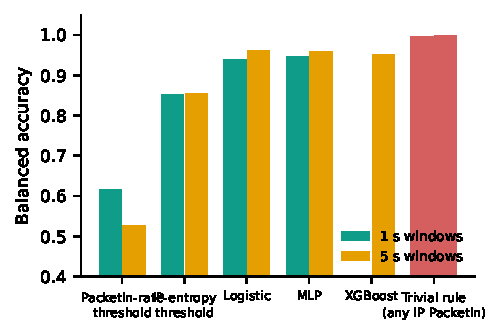
\includegraphics[width=\columnwidth]{fig_scores.pdf}
\caption{Balanced accuracy on unseen captures, capture-grouped CV, 10 seeds (XGBoost was run at 5\,s only). The red bars are the trivial rule ``at least one IP PacketIn'' scored inside attack sessions, which matches or exceeds every model. Data: \texttt{v4\_strict\_W1.json}, \texttt{v4\_strict\_W5\_xgb.json}, \texttt{review\_checks.json}.}\label{fig:scores}
\end{figure}

\textbf{With broader labels the margin over the trivial rule is real but not clean.} Under the IP-based label rule
(\S\ref{sec:discussion}), which keeps all windows, the same trivial rule scores 0.741 pooled and 0.700 macro at 1\,s
(0.653 and 0.668 at 5\,s), while the MLP scores 0.794 and 0.855 (0.715 and 0.782). The MLP is ahead, but this rule
labels windows by IP membership, which overlaps with the IP-count features, so the comparison is not independent.

\textbf{The session probe is too small and too impure to quantify session identity (Table~\ref{tab:confound}).} We
remove attack-matched PacketIns, drop controller-reply counts, keep windows with at least five remaining PacketIns, and
train the MLP to predict whether a window comes from an attack session. It reaches BAcc 0.940 (majority 0.500), but the
attack side has 518 windows, of which 424 (82\%) contain unmatched-IP PacketIns that may simply be attack traffic the
CSV does not list; the stricter variant using only attack-free windows has 6 windows from 2 captures at 1\,s (0.950)
and 2 windows at 5\,s (0.550). Under the IP-based rule the corresponding probe scores 0.806 and 0.783, again with
unlisted traffic in the ``attack-free'' class. We conclude only that the available data cannot rule out
session-recognition as a source of the scores; we do not claim that sessions are separable independently of attack
traffic.

\subsection{Evaluation-validity audit: random flow splits versus held-out hosts}\label{sec:audit}
\textbf{What is already known.} That randomised train/test splits and identifier columns (Flow ID, IPs, ports, timestamps) can inflate NIDS scores
has been argued for non-SDN benchmarks: Engelen et al.~\cite{engelen2021troubleshooting} warn that identifier columns let a model associate
host-specific information with a class, and Flood et al.~\cite{flood2024baddesign} show, on seven datasets that include CICIDS2017 but no SDN dataset, that standard
randomised splits leak because of homogeneous traffic. We do not claim the phenomenon. In the papers we could read we found no study that measures it on
InSDN or another SDN dataset, and none that reports a paired grouped-versus-random accuracy gap with confidence intervals for two datasets under one
pipeline (a limited search, not proof of absence).

\textbf{What we add.} We ran one pipeline on two datasets: XGBoost on the GPU, 77 numeric CICFlowMeter features without IPs, ports or timestamps,
benign versus attack, 10 seeds (Table~\ref{tab:audit}, Fig.~\ref{fig:split}). A random stratified 70:30 flow split gives balanced accuracy 0.9998 on InSDN (343\,889 flows)
and 0.9917 on CICIDS2017 (2\,100\,814 flows). Holding out source hosts (70:30 by source IP, no host in both sets) gives $0.907\pm0.085$ on InSDN, with
individual splits from 0.66 to 1.00, and $0.641\pm0.056$ on CICIDS2017. A per-file time-ordered split shows no drop on InSDN (0.9997), so there the effect
works through hosts and not through adjacent flows, but it falls to 0.719 on CICIDS2017, so no single explanation covers both. A classifier given only IP
addresses, ports and the Flow ID scores at least 0.9999 on both datasets, so identity alone separates the classes. As a measure of redundancy, 48.7\% of
the random-split test rows on InSDN (20.3\% on CICIDS2017) have an exact duplicate of their full feature vector in the training set. Redundancy is not the mechanism: dropping all exact duplicates (343,889 to 184,607 rows) leaves the random-split score at 0.9998, and holding out source hosts while requiring every attack class to appear in training still gives 0.939 (0.812 after de-duplication), so the drop is not a missing-class artefact; splitting by the source--destination--port triple instead gives 0.961 (0.984 de-duplicated), so the effect is tied to unseen source hosts rather than to flows in general. A partial replication of one published pipeline (SDNGuardStack, our approximation, five seeds, default hyperparameters) reproduces its reported accuracy under a random split (0.9999 against the reported 99.98\%) but not under held-out hosts (0.72--0.78, 95\% CI up to $\pm$0.39), so the published number is reproducible and the question is what it measures. We also tried a third
dataset, UKMDDoSDN~\cite{ukmddosdn2025}, but it was skipped: its two public PCAPs contain no benign class (Appendix~\ref{app:ukm}).

\textbf{What we can and cannot say about published InSDN papers.} We examined 12 papers (eleven on SDN or InSDN-related data, one on other benchmarks) and
read 10 in full (\texttt{literature\_check.json}); the other two are characterised by their abstracts only and we make no claim about their methods.
Of the nine InSDN papers read in full, none reports a host-grouped or capture-grouped split, and three use identifier columns (such as Flow ID or source IP) among their model inputs;
the remaining papers either state that they removed such columns or do not say. This means their protocols cannot rule out the leakage we measure. It does not show that any
reported number is wrong: we use our own classifier and the CSV features, and did not re-run any cited model.

\textbf{Recipe replication with one classifier.} To see whether the gap depends on which features are used, we ran four feature recipes on InSDN with the same XGBoost (80:20 splits, 10 seeds, Table~\ref{tab:recipe}): numeric flow features only, numeric plus ports, numeric plus identifier columns, and the 15 features with highest mutual information selected on all rows before the split. These approximate feature choices described in published InSDN papers; they are not those papers' models, code or reported numbers, and we do not claim to have reproduced them. Under a random split every recipe reaches binary balanced accuracy of at least 0.9998 and 8-class accuracy of at least 0.9991. Under a source-IP-grouped split binary balanced accuracy falls to between 0.856 and 0.943 and 8-class accuracy to between 0.687 and 0.835, with wide intervals (up to $\pm$0.241). Adding ports lowered the grouped score (0.856 against 0.943 for numeric features only), and adding identifier columns changed it little (0.941), so on this classifier identifiers neither rescue nor much hurt grouped performance. The mutual-information selection, run before the split, picked Flow ID, Src IP and Dst IP among its 15 features. Grouping by source IP also changes the attack-class composition between train and test, so the grouped numbers are a stress test and not ``the true accuracy''; the protocol cannot rule out that published random-split scores would fall under host-grouped evaluation, and it does not show that they would.

\begin{figure}[t]
\centering
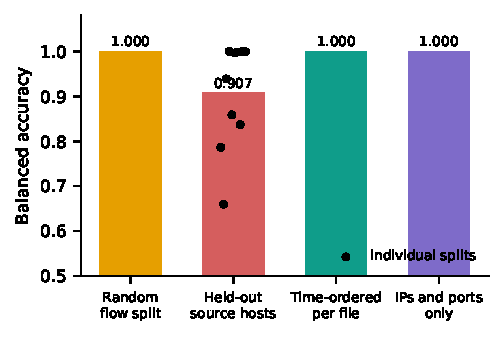
\includegraphics[width=\columnwidth]{fig_split.pdf}
\caption{Same classifier and features under four evaluation protocols on two datasets (benign vs.\ attack, 10 seeds). Dots are the ten source-host splits. Data: \texttt{protocol\_audit\_insdn.json}, \texttt{protocol\_audit\_cicids2017.json}.}\label{fig:split}
\end{figure}

\textbf{Consequence for the controller-view scores.} The headline scores of \S\ref{sec:results} are feasibility evidence that PacketIn-level features
distinguish InSDN's attack captures from its benign captures, not a measurement of attack-detection accuracy. A
convincing evaluation needs benign and attack traffic interleaved within one session, with labels for all
controller-visible traffic, which InSDN does not provide.

\section{A Forwarding-Application Case Study}\label{sec:live}
InSDN shows one forwarding configuration. To see whether what the controller observes depends on the forwarding
application, we built a small testbed (Mininet, one Open vSwitch switch, six hosts; a Ryu OpenFlow~1.3 learning
switch with a configurable entry granularity) and recorded its control channel with the same parser. The three modes
install, for each learned destination, an entry matching (i) the MAC pair; (ii) the 5-tuple for TCP/UDP with a 10\,s
idle timeout; or (iii) the 5-tuple with a 2\,s idle timeout applied to all entries. In the two 5-tuple modes, other IP
traffic receives an (src, dst, protocol) entry and ARP an ARP-only entry, so a coarse entry for one protocol cannot
match another. The controller polls flow statistics every second. Traffic is benign only and generated by the same
program with the same random seeds in every mode (request timing still differs): five hosts repeatedly fetch files of
16\,KB to 1\,MB from an HTTP server (80\%) or ping it (20\%) with random pacing for 90\,s (captures span
$\sim$99\,s including start-up). Each mode was run 5 times, reporting mean and 95\% $t$-interval over runs
(Table~\ref{tab:live}); the 15 runs completed 13\,366 requests, of which 41 failed (below).

\begin{table*}[t]
\caption{Forwarding application vs.\ what the controller observes: benign traffic from the same generator and seeds (5 hosts $\rightarrow$ 1 HTTP server, plus pings), 1-switch Mininet/Ryu testbed, $\sim$99\,s capture per run, 10 runs per mode, mean{\scriptsize$\pm$}95\% CI. Entries = flow entries returned per flow-statistics reply (1\,s polling). }
\label{tab:live}
\centering\small
\begin{tabular}{lccccc}
\toprule
Mode & TCP PacketIns & All PacketIns & FlowMods & MAC-pair entries & IP-specific entries \\
\midrule
MAC-pair (as ONOS in InSDN) & 12.3{\scriptsize$\pm$2.3} & 76.8{\scriptsize$\pm$1.8} & 19.1{\scriptsize$\pm$1.8} & 9.5{\scriptsize$\pm$0.0} & 0.0{\scriptsize$\pm$0.0} \\
5-tuple, 10\,s idle & 10422.0{\scriptsize$\pm$202.0} & 10497.0{\scriptsize$\pm$204.7} & 10442.8{\scriptsize$\pm$200.8} & 0.0{\scriptsize$\pm$0.0} & 153.1{\scriptsize$\pm$2.4} \\
5-tuple, 2\,s idle & 10391.6{\scriptsize$\pm$249.4} & 10611.3{\scriptsize$\pm$258.7} & 10556.4{\scriptsize$\pm$252.3} & 0.0{\scriptsize$\pm$0.0} & 36.9{\scriptsize$\pm$0.5} \\
\bottomrule
\end{tabular}
\end{table*}


\textbf{Granularity sets the PacketIn volume.} MAC-pair mode produced $11.6\pm4.2$ TCP PacketIns per run, against
$10\,350\pm440$ (10\,s idle) and $10\,233\pm415$ (2\,s idle) under per-flow forwarding: 675$\times$ to 1\,752$\times$ (10\,s idle)
and 685$\times$ to 1\,780$\times$ (2\,s idle) more in each of the five paired runs (larger in 5 of 5; the smallest possible two-sided sign-test $p$ at five pairs is
0.0625, but the intervals are separated by nearly three orders of magnitude). That is about 11--12 TCP PacketIns per
completed request, so each connection is punted repeatedly; the most likely cause is packets that arrive before the
FlowMod takes effect (we install entries without a barrier and send full packets), but we did not isolate this
mechanism. FlowMods (18.8 vs.\ about 10\,380 per run) track the PacketIns and are not independent evidence. The
MAC-pair result is a replication: the same mode in the first, flawed campaign gave $11.0\pm4.1$.

\textbf{Idle timeout sets what a poller sees.} Per-flow entries returned per statistics reply fell from $151.9\pm1.8$
to $36.8\pm0.4$ when the idle timeout dropped from 10\,s to 2\,s, a ratio of 0.239 to 0.246 in all five pairs: entries
expire between polls, so a 1\,s poller sees about a quarter as many. The result is close to what a shorter timeout
implies; its value is the size of the loss for a realistic polling interval. In MAC-pair mode the replies contain only
the table-miss rule and MAC-pair entries ($9.5\pm0.1$ per reply); no entry matches IP or transport fields, as in
InSDN (whose ONOS additionally installed \texttt{eth\_type} punt rules).

\textbf{A flawed first campaign.} Our first application installed MAC-pair entries for ping and ARP in every mode;
these also match later TCP between the same hosts, so most connections never reached the controller and per-flow mode
produced only $43.4\pm30.1$ TCP PacketIns per run (4$\times$ MAC-pair) with a wide interval. The original application
is archived as \texttt{ryu\_fwd\_v1.py}. We report it because it shows how an overlapping coarse entry hides traffic
from the controller by two orders of magnitude, independently of the forwarding mode's nominal granularity.

\textbf{Reliability.} One run (5-tuple, 2\,s idle, seed 4) had 41 failed requests (7--10 per client); the other 14
runs had none. With about $10^4$ PacketIns per run the controller may have been overloaded; we did not investigate and
include the run in all figures.

\textbf{Scope.} This is a single-switch testbed with one forwarding application and benign traffic only; we run no
attacks or detectors in it. The mode contrast does not transfer to InSDN's ONOS, which punted about one packet per
target packet even with MAC-pair entries (\S\ref{sec:gap}), and no claim is made about detection accuracy under any
forwarding mode.


\section{Discussion and Limitations}\label{sec:discussion}
\textbf{Scope of the audit.} The audit is offline and uses flow-CSV features: we did not replay interleaved live traffic, and the grouped splits
(by source IP) are one of several possible groupings. It uses XGBoost only; other models may be affected differently. Source-IP grouping also removes
attacker identity, so lower grouped scores partly reflect genuinely harder generalisation to unseen attackers and not only leakage; we do not separate the two. A third dataset, UKMDDoSDN, could not be
used (two PCAPs, no benign class), so two datasets is the evidence base. Time-ordered and grouped results disagree across the two datasets (Table~\ref{tab:audit}), and we have not identified why.

\textbf{Single testbed.} All InSDN controller-view results come from one ONOS/OVS deployment with 44 controller captures; class
counts are small for exploit, web, brute force and botnet. Confidence intervals reflect fold and initialisation
variability, not new testbeds.

\textbf{Forwarding-application dependence.} The observability gap follows from ONOS reactive forwarding as
configured in InSDN. An application installing 5-tuple entries would expose finer counters at higher flow-table cost,
and the PacketIn stream would then be sparser. Our pipeline measures the gap for any capture; the numbers are
specific to this configuration.

\textbf{Labels.} Strict labels leave brute force, exploit, web and DDoS with few attack windows because the CSV
omits much of their traffic (for DDoS, most of the spoofed flood). An alternative rule that also counts IPs seen only
in attack flows labels more windows but overlaps with the IP-count features, so we report it as a sensitivity
analysis. Under that broader rule overall BAcc is lower (MLP 0.881, logistic regression 0.847, best threshold 0.748 at
1\,s; MLP 0.887, best threshold 0.769 at 5\,s) and within-session macro BAcc is 0.855 (0.782 at 5\,s). The ranking
against thresholds is unchanged, and at 1\,s the MLP is ahead of the best threshold on flood, web and brute force,
level on probe (0.812 vs.\ 0.794, within the interval) and behind on exploit and botnet. Transfer from Metasploitable-2 to OVS no longer
beats the best threshold (0.678 vs.\ 0.678), while OVS to Metasploitable-2 remains strong (0.977 vs.\ 0.924).

\textbf{Published-paper check.} Our comparison of split protocols uses our own classifier and the CSV features; it shows the random-split protocol
overstates held-out-host performance on InSDN by about nine points (and on CICIDS2017 by about 35), not that any author's reported number is wrong. We read 10 of 12 examined papers in full (nine of them on InSDN); no
published model was re-run, and the two unread papers are not characterised.

\textbf{Baselines and deployment.} A GPU gradient-boosted tree baseline (XGBoost, BAcc $0.952\pm0.013$ at 5\,s, strict labels, 10 seeds) does not beat the linear ($0.961\pm0.011$) or MLP ($0.958\pm0.012$) models; detection is run offline on recorded control channels,
not inline in a live controller, and we do not measure controller-side latency or mitigation effects. The forwarding
study (\S\ref{sec:live}) uses benign traffic and at most three switches; it measures visibility, not detection, and a
cross-testbed detection experiment with labelled attacks is future work.

\textbf{Deployment.} A controller-side detector of this kind would run beside the control channel, reading a port mirror or the
controller's message log, and would need the forwarding application's granularity to be stable: switching from MAC-pair to per-flow
forwarding changed TCP PacketIn volume by two to three orders of magnitude in our testbed, so any threshold or model tied to PacketIn
rates must be retrained, or at least recalibrated, after a forwarding change. The idle timeout also changes what a poller sees
(about a quarter as many per-flow entries at 2\,s as at 10\,s). Per-flow forwarding exposes finer counters at a controller-load and
flow-table cost that we did not measure. Missing before deployment can be argued: interleaved benign and attack traffic in one session,
a second controller family beyond Ryu applications (OpenDaylight, ONOS under other applications), and online latency.

\textbf{What we could not do.} We did not re-implement a published controller-side detector from its paper, so the comparison
is to threshold heuristics and our own models only. The two public candidates we examined as second sources
(Appendix~\ref{app:ukm}) could not be used.

\section{Conclusion}
InSDN's own controller never installed or reported the 5-tuple flow entries InSDN labels: its flow entries are MAC
pairs or EtherType rules, and its view of traffic is a PacketIn stream. Restricted to that view, small models separate InSDN's attack
captures from its benign captures on unseen captures, withheld families and a second deployment, where the usual
PacketIn-rate heuristic does not (BAcc 0.946 vs.\ 0.616 on unseen captures). We could not show that this reflects
attack detection rather than session recognition and label coverage: within sessions a trivial IP-PacketIn rule
matches or beats the model under strict labels, and our probes lack clean attack-free windows. We therefore present
controller-observable evaluation on InSDN as feasible but unproven, and recommend datasets that interleave benign and
attack traffic. A benign-traffic Mininet/Ryu study shows that forwarding-application choices (entry granularity, idle
timeout) change what the controller can observe. The pipeline, capture hashes and result files accompany this paper.

\appendices
\section{Candidate Second Datasets Examined}\label{app:ukm}
UKMDDoSDN~\cite{ukmddosdn2025}: we downloaded \texttt{syn\_flood\_combined.pcap} (18\,922\,240\,B; 199\,273 packets) and
\texttt{udp\_flood\_combined.pcap} (15\,420\,748\,B; 110\,518 packets) from the authors' repository, parsed them (pcapng, Linux cooked v2) and found no
packet on TCP port 6633 or 6653: they are data-plane captures from many per-host interfaces. The CSV files the dataset page
describes were not in the repository listing and the Mendeley file list could not be read, so we make no claim about them. The
dataset page states CC BY 4.0 while the repository is MIT-licensed; we did not resolve this. LAN-SDN-NIDS~\cite{lansdnnids2026}: we
read its Crossref record (the publisher page refused automated access), which describes a flow-level dataset of 1\,125\,059 records with
11 control-plane metrics; we could not verify whether raw OpenFlow captures are released, and flow-level counts of PacketIn and FlowMod
would not expose FlowMod match fields. Neither was used as data. Hashes are in \texttt{data/MANIFEST.md}.

\section*{Data and Code Availability}\label{sec:avail}
The InSDN CSVs and PCAPs are public (sources and SHA-256 hashes in \texttt{data/MANIFEST.md}). Our parser, feature extraction,
experiments, forwarding-study applications, result files and table generators are in the project repository; the script
\texttt{research/insdn\_controller/reproduce.sh} rebuilds the features from the raw ONOS captures, re-runs every experiment, and
compares each result file with the stored one (tolerance $10^{-6}$), and \texttt{paper/verify\_numbers.py} checks the numbers quoted in the
text against the result files. Hashes of every capture we recorded are in \texttt{capture\_hashes.sha256}. Re-recording the live
captures needs root privileges and will not reproduce packet timing exactly. The first, flawed campaign's captures were not retained;
only its summary file is.

\section*{Acknowledgment}
All three authors contributed equally to the data analysis, experiments and writing.

\bibliographystyle{IEEEtran}
\bibliography{references}
\end{document}
